\let\negmedspace\undefined
\let\negthickspace\undefined
\documentclass[journal]{IEEEtran}
\usepackage[a5paper, margin=10mm, onecolumn]{geometry}
%\usepackage{lmodern} 
\usepackage{tfrupee} 

\setlength{\headheight}{1cm} 
\setlength{\headsep}{0mm}     

\usepackage{gvv-book}
\usepackage{gvv}
\usepackage{cite}
\usepackage{amsmath,amssymb,amsfonts,amsthm}
\usepackage{algorithmic}
\usepackage{graphicx}
\usepackage{textcomp}
\usepackage{xcolor}
\usepackage{txfonts}
\usepackage{listings}
\usepackage{enumitem}
\usepackage{mathtools}
\usepackage{gensymb}
\usepackage{comment}
\usepackage[breaklinks=true]{hyperref}
\usepackage{tkz-euclide} 
\usepackage{listings}                                        
\def\inputGnumericTable{}                                 
\usepackage[latin1]{inputenc}                                
\usepackage{color}                                            
\usepackage{array}                                            
\usepackage{longtable}                                       
\usepackage{calc}                                             
\usepackage{multirow}                                         
\usepackage{hhline}                                           
\usepackage{ifthen}                                           
\usepackage{lscape}

\begin{document}

\bibliographystyle{IEEEtran}
\vspace{3cm}

\title{1.6.18}
\author{AI25BTECH11003 - Bhavesh Gaikwad}
{\let\newpage\relax\maketitle}

\renewcommand{\thefigure}{\theenumi}
\renewcommand{\thetable}{\theenumi}
\setlength{\intextsep}{10pt} 


\numberwithin{equation}{enumi}
\numberwithin{figure}{enumi}
\renewcommand{\thetable}{\theenumi}


\textbf{Question}: Prove that points A(2,1), B(0,5) and C(-1,2) are not collinear.\\\\

\textbf{Solution:}\\

$\vec{B}-\vec{A}$=$\myvec{0-2 \\ 5-1}$ = $\myvec{-2 \\ 4}$
$\qquad \vec{C}-\vec{A}=\myvec{-1-2 \\ 2-1}$ =$\myvec{-3 \\ 1}$ \\
$\vec{M}$ = $\myvec{\vec{B}-\vec{A} & \vec{C}-\vec{A}}^T$ = $\myvec{-2 & -3 \\ 4 & 1}$\\\\

Row-reduce to compute the rank:\\

$\myvec{-2 & -3\\ 4 & 1}$ $\xrightarrow{\;R_2\leftarrow R_2+2R_1\;}$ $\myvec{-2 & -3 \\ 0 & -5}$\\

The echelon form has two nonzero rows, hence
rank(M)=2$\neq$1

\begin{align}
    \centering
    \boxed{Therefore, \, The \, points \, A(2,1), \,B(0,5) \, and \, C(-1,2) \, are \, not \, collinear.}
\end{align}
\bigskip

\begin{figure}[htbp]
    \centering
    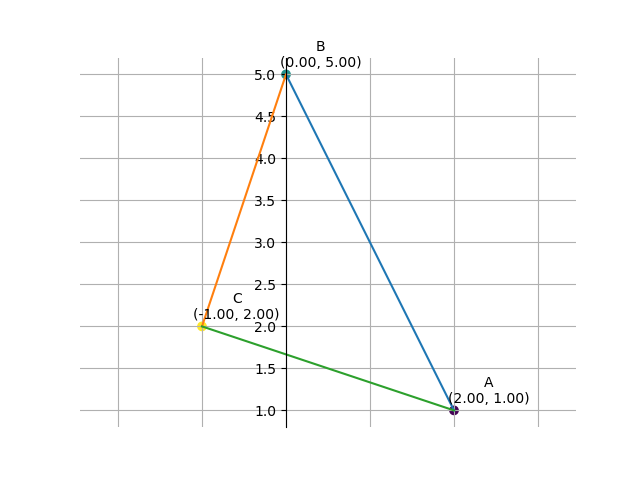
\includegraphics[width=0.8\linewidth]{figs/fig1.png}
    \caption{Graph}
    \label{fig:fig/fig1.png}
\end{figure}
\end{document}  
